\documentclass{standalone}
\usepackage{tikz}
\usetikzlibrary{patterns, positioning}
\usepackage[sfdefault]{ClearSans} %% option 'sfdefault' activates Clear Sans as the default text font
\usepackage[T1]{fontenc}

\begin{document}
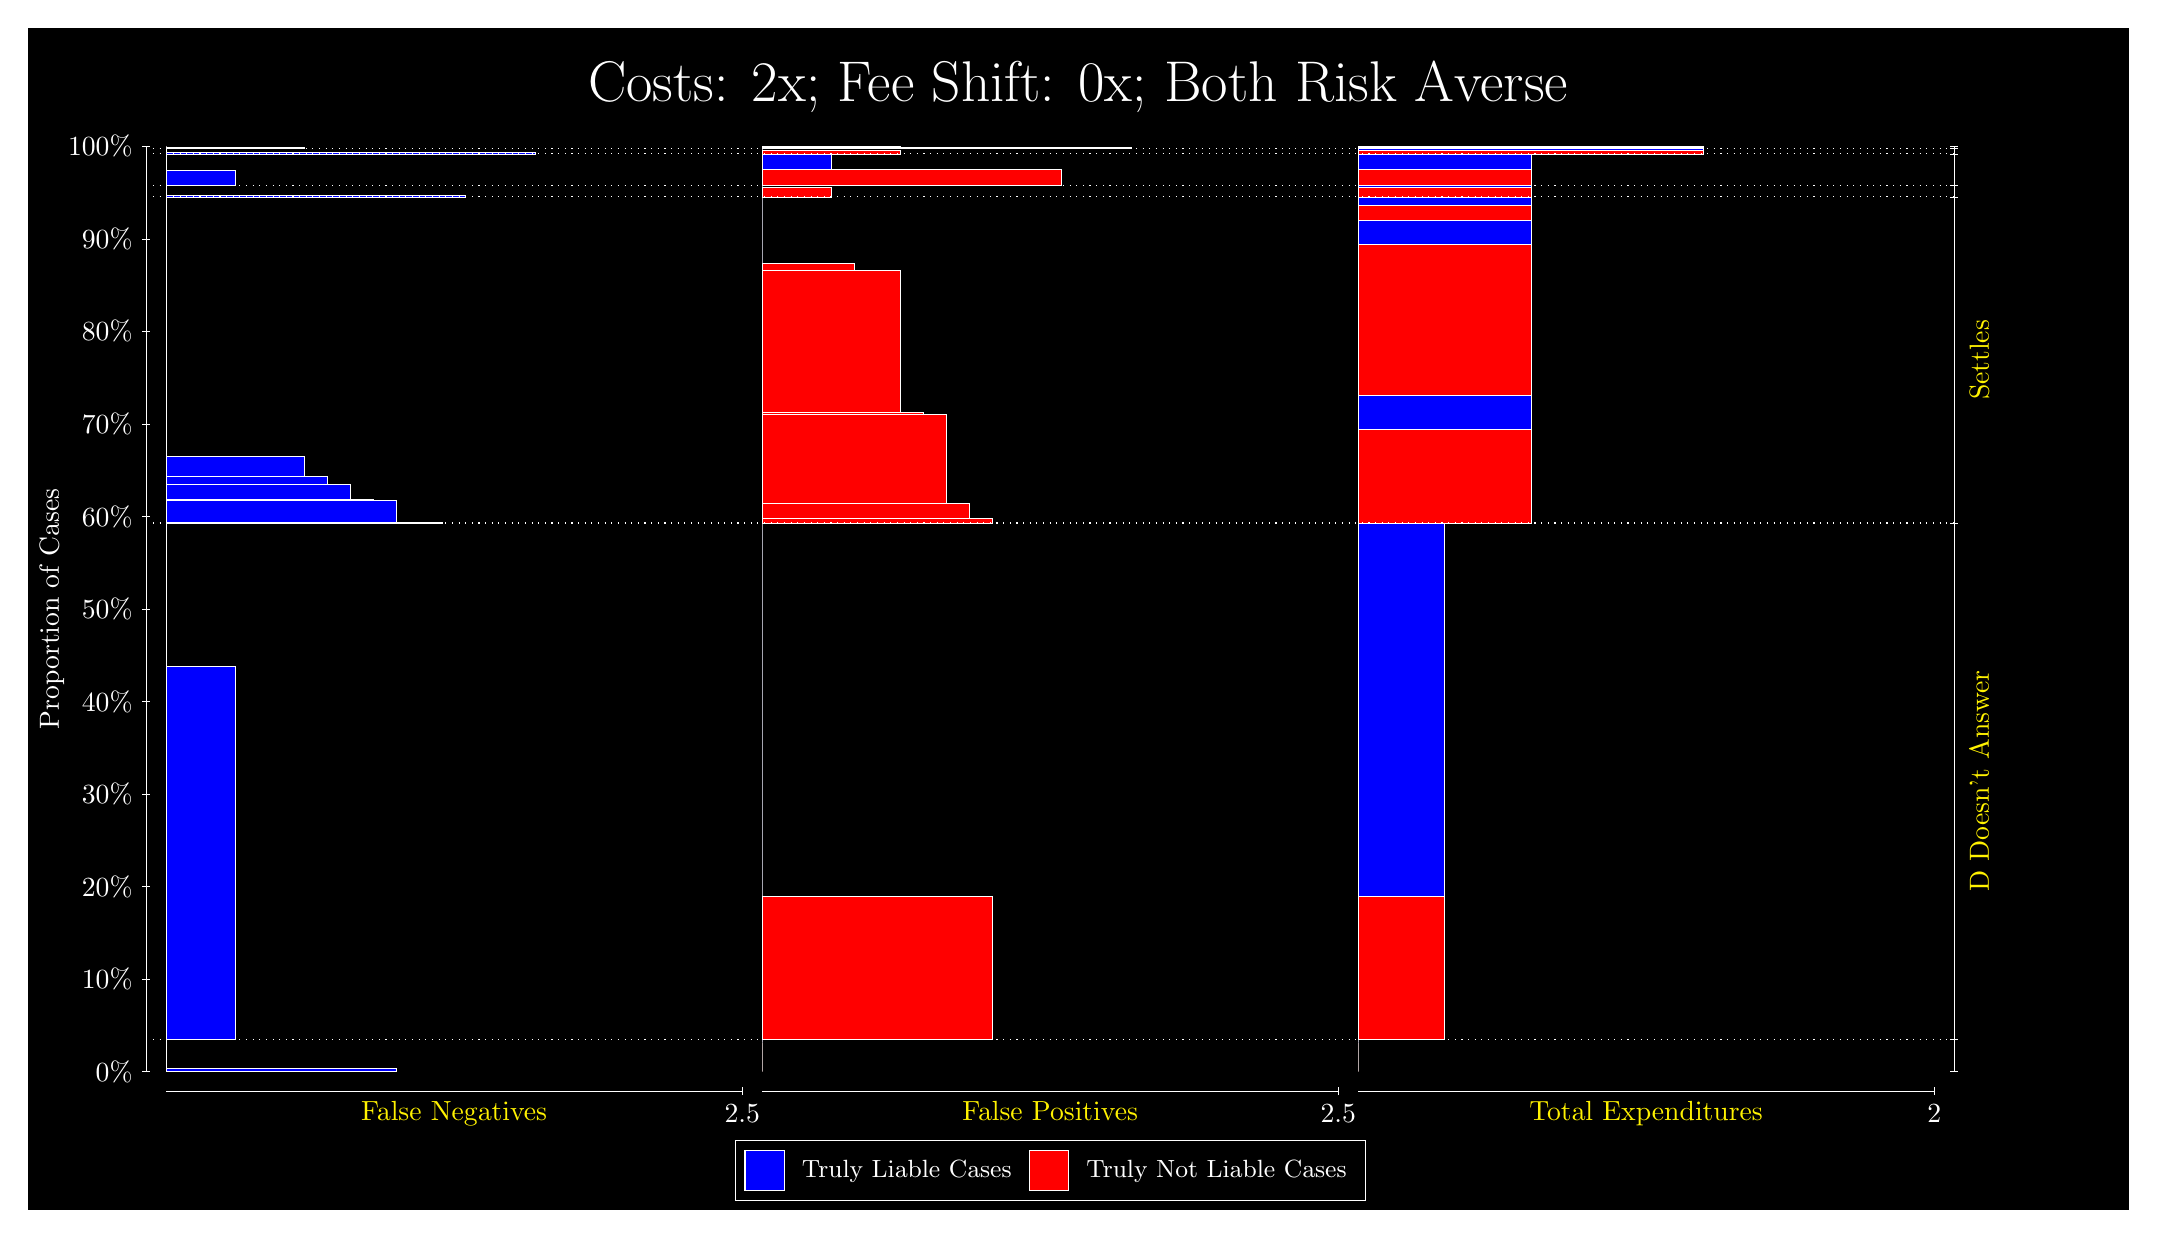
\begin{tikzpicture}
\draw[fill=black] (0,0) rectangle (26.667,15);
\draw[text=white] (0,13.5) rectangle (26.667,15) node[midway] {\huge Costs: 2x; Fee Shift: 0x; Both Risk Averse};
\draw[white, very thin] (1.5,1.75) -- (1.5,13.5);
\node[rotate=90, text=white, anchor=center] at (0.3, 7.625) {Proportion of Cases};
\draw[white, very thin] (1.45,1.75) -- (1.55,1.75);
\node[text=white, anchor=east] at (1.45, 1.75) {0\%};
\draw[white, very thin] (1.45,2.925) -- (1.55,2.925);
\node[text=white, anchor=east] at (1.45, 2.925) {10\%};
\draw[white, very thin] (1.45,4.1) -- (1.55,4.1);
\node[text=white, anchor=east] at (1.45, 4.1) {20\%};
\draw[white, very thin] (1.45,5.275) -- (1.55,5.275);
\node[text=white, anchor=east] at (1.45, 5.275) {30\%};
\draw[white, very thin] (1.45,6.45) -- (1.55,6.45);
\node[text=white, anchor=east] at (1.45, 6.45) {40\%};
\draw[white, very thin] (1.45,7.625) -- (1.55,7.625);
\node[text=white, anchor=east] at (1.45, 7.625) {50\%};
\draw[white, very thin] (1.45,8.8) -- (1.55,8.8);
\node[text=white, anchor=east] at (1.45, 8.8) {60\%};
\draw[white, very thin] (1.45,9.975) -- (1.55,9.975);
\node[text=white, anchor=east] at (1.45, 9.975) {70\%};
\draw[white, very thin] (1.45,11.15) -- (1.55,11.15);
\node[text=white, anchor=east] at (1.45, 11.15) {80\%};
\draw[white, very thin] (1.45,12.325) -- (1.55,12.325);
\node[text=white, anchor=east] at (1.45, 12.325) {90\%};
\draw[white, very thin] (1.45,13.5) -- (1.55,13.5);
\node[text=white, anchor=east] at (1.45, 13.5) {100\%};

\draw[white, very thin] (24.457,1.75) -- (24.457,13.5);
\draw[white, very thin] (24.407,1.75) -- (24.507,1.75);
\node[anchor=west] at (24.407, 1.75) {};
\draw[white, very thin] (24.407,2.1599) -- (24.507,2.1599);
\node[anchor=west] at (24.407, 2.1599) {};
\draw[white, very thin] (24.407,8.7169) -- (24.507,8.7169);
\node[anchor=west] at (24.407, 8.7169) {};
\draw[white, very thin] (24.407,12.859) -- (24.507,12.859);
\node[anchor=west] at (24.407, 12.859) {};
\draw[white, very thin] (24.407,13.002) -- (24.507,13.002);
\node[anchor=west] at (24.407, 13.002) {};
\draw[white, very thin] (24.407,13.405) -- (24.507,13.405);
\node[anchor=west] at (24.407, 13.405) {};
\draw[white, very thin] (24.407,13.471) -- (24.507,13.471);
\node[anchor=west] at (24.407, 13.471) {};
\draw[white, very thin] (24.407,13.5) -- (24.507,13.5);
\node[anchor=west] at (24.407, 13.5) {};

\draw[white, very thin, fill=blue] (1.75,1.75) rectangle (4.6775,1.7931);
\draw[white, very thin, fill=red] (1.75,1.7931) rectangle (1.75,2.1599);
\draw[white, very thin, fill=blue] (1.75,2.1599) rectangle (2.6283,6.8983);
\draw[white, very thin, fill=red] (1.75,6.8983) rectangle (1.75,8.7169);
\draw[white, very thin, fill=blue] (1.75,8.7169) rectangle (5.2631,8.7313);
\draw[white, very thin, fill=blue] (1.75,8.7313) rectangle (4.6775,9.011);
\draw[white, very thin, fill=blue] (1.75,9.011) rectangle (4.3848,9.0207);
\draw[white, very thin, fill=blue] (1.75,9.0207) rectangle (4.092,9.2057);
\draw[white, very thin, fill=blue] (1.75,9.2057) rectangle (3.7993,9.3087);
\draw[white, very thin, fill=blue] (1.75,9.3087) rectangle (3.5065,9.564);
\draw[white, very thin, fill=red] (1.75,9.564) rectangle (1.75,12.859);
\draw[white, very thin, fill=blue] (1.75,12.859) rectangle (5.5558,12.88);
\draw[white, very thin, fill=red] (1.75,12.88) rectangle (1.75,13.002);
\draw[white, very thin, fill=blue] (1.75,13.002) rectangle (2.6283,13.198);
\draw[white, very thin, fill=red] (1.75,13.198) rectangle (1.75,13.405);
\draw[white, very thin, fill=blue] (1.75,13.405) rectangle (6.4341,13.42);
\draw[white, very thin, fill=red] (1.75,13.42) rectangle (1.75,13.471);
\draw[white, very thin, fill=blue] (1.75,13.471) rectangle (3.5065,13.485);
\draw[white, very thin, fill=red] (1.75,13.485) rectangle (1.75,13.5);
\draw[white, very thin, fill=red] (9.3189,1.75) rectangle (9.3189,2.1168);
\draw[white, very thin, fill=blue] (9.3189,2.1168) rectangle (9.3189,2.1599);
\draw[white, very thin, fill=red] (9.3189,2.1599) rectangle (12.246,3.9785);
\draw[white, very thin, fill=blue] (9.3189,3.9785) rectangle (9.3189,8.7169);
\draw[white, very thin, fill=red] (9.3189,8.7169) rectangle (12.246,8.7793);
\draw[white, very thin, fill=red] (9.3189,8.7793) rectangle (11.954,8.9702);
\draw[white, very thin, fill=red] (9.3189,8.9702) rectangle (11.661,10.091);
\draw[white, very thin, fill=red] (9.3189,10.091) rectangle (11.368,10.127);
\draw[white, very thin, fill=red] (9.3189,10.127) rectangle (11.075,11.922);
\draw[white, very thin, fill=red] (9.3189,11.922) rectangle (10.49,12.012);
\draw[white, very thin, fill=blue] (9.3189,12.012) rectangle (9.3189,12.859);
\draw[white, very thin, fill=red] (9.3189,12.859) rectangle (10.197,12.981);
\draw[white, very thin, fill=blue] (9.3189,12.981) rectangle (9.3189,13.002);
\draw[white, very thin, fill=red] (9.3189,13.002) rectangle (13.125,13.208);
\draw[white, very thin, fill=blue] (9.3189,13.208) rectangle (10.197,13.405);
\draw[white, very thin, fill=red] (9.3189,13.405) rectangle (11.075,13.456);
\draw[white, very thin, fill=blue] (9.3189,13.456) rectangle (9.3189,13.471);
\draw[white, very thin, fill=red] (9.3189,13.471) rectangle (14.003,13.485);
\draw[white, very thin, fill=blue] (9.3189,13.485) rectangle (11.075,13.5);
\draw[white, very thin, fill=red] (16.888,1.75) rectangle (16.888,2.1168);
\draw[white, very thin, fill=blue] (16.888,2.1168) rectangle (16.888,2.1599);
\draw[white, very thin, fill=red] (16.888,2.1599) rectangle (17.986,3.9785);
\draw[white, very thin, fill=blue] (16.888,3.9785) rectangle (17.986,8.7169);
\draw[white, very thin, fill=red] (16.888,8.7169) rectangle (19.083,9.9003);
\draw[white, very thin, fill=blue] (16.888,9.9003) rectangle (19.083,10.341);
\draw[white, very thin, fill=red] (16.888,10.341) rectangle (19.083,12.261);
\draw[white, very thin, fill=blue] (16.888,12.261) rectangle (19.083,12.565);
\draw[white, very thin, fill=red] (16.888,12.565) rectangle (19.083,12.756);
\draw[white, very thin, fill=blue] (16.888,12.756) rectangle (19.083,12.859);
\draw[white, very thin, fill=red] (16.888,12.859) rectangle (19.083,12.981);
\draw[white, very thin, fill=blue] (16.888,12.981) rectangle (19.083,13.002);
\draw[white, very thin, fill=red] (16.888,13.002) rectangle (19.083,13.208);
\draw[white, very thin, fill=blue] (16.888,13.208) rectangle (19.083,13.405);
\draw[white, very thin, fill=red] (16.888,13.405) rectangle (21.279,13.456);
\draw[white, very thin, fill=blue] (16.888,13.456) rectangle (21.279,13.471);
\draw[white, very thin, fill=red] (16.888,13.471) rectangle (21.279,13.485);
\draw[white, very thin, fill=blue] (16.888,13.485) rectangle (21.279,13.5);
\draw[white, dotted] (1.5,2.1599) -- (24.457,2.1599);
\draw[white, dotted] (1.5,8.7169) -- (24.457,8.7169);
\draw[white, dotted] (1.5,12.859) -- (24.457,12.859);
\draw[white, dotted] (1.5,13.002) -- (24.457,13.002);
\draw[white, dotted] (1.5,13.405) -- (24.457,13.405);
\draw[white, dotted] (1.5,13.471) -- (24.457,13.471);
\draw[white, very thin] (1.75,1.5) -- (9.0689,1.5);
\node[text=yellow, anchor=north] at (5.4094, 1.5) {False Negatives};
\draw[white, very thin] (9.0689,1.45) -- (9.0689,1.55);
\node[text=white, anchor=north] at (9.0689, 1.45) {2.5};

\draw[white, very thin] (9.3189,1.5) -- (16.638,1.5);
\node[text=yellow, anchor=north] at (12.978, 1.5) {False Positives};
\draw[white, very thin] (16.638,1.45) -- (16.638,1.55);
\node[text=white, anchor=north] at (16.638, 1.45) {2.5};

\draw[white, very thin] (16.888,1.5) -- (24.207,1.5);
\node[text=yellow, anchor=north] at (20.547, 1.5) {Total Expenditures};
\draw[white, very thin] (24.207,1.45) -- (24.207,1.55);
\node[text=white, anchor=north] at (24.207, 1.45) {2};


\node[text=yellow, centered, rotate=90] at (24.777, 5.4384) {D Doesn't Answer};
\node[text=yellow, centered, rotate=90] at (24.777, 10.788) {Settles};





\draw (12.978300999999998,1.5) node[draw=none] (baseCoordinate) {};
\begin{scope}[align=center]
        \matrix[scale=0.5, draw=white, below=0.5cm of baseCoordinate, nodes={draw}, column sep=0.1cm]{
            \node[rectangle, draw, minimum width=0.5cm, minimum height=0.5cm, fill=blue] {}; &
            \node[draw=none, font=\small, text=white] (B) {Truly Liable Cases}; &
            \node[rectangle, draw, minimum width=0.5cm, minimum height=0.5cm, fill=red] {}; &
            \node[draw=none, font=\small, text=white] (B) {Truly Not Liable Cases}; \\
            };
\end{scope}

\end{tikzpicture}
\end{document}